\documentclass[conference]{IEEEtran}
\IEEEoverridecommandlockouts

%% --- Paquetes ---
\usepackage[utf8]{inputenc}
\usepackage[T1]{fontenc}
\usepackage[spanish,es-nodecimaldot]{babel}
\usepackage{amsmath,amssymb}

%% Comandos propios
\newcommand{\NP}{\ensuremath{\mathcal{NP}}}
\DeclareMathOperator*{\argmin}{arg\,min}
\usepackage{booktabs}
\usepackage{multirow}
\usepackage{graphicx}
\usepackage{url}
\usepackage{hyperref}
\usepackage{xcolor}
\usepackage{algorithm}
\usepackage{algpseudocode}
%% Entrada/salida de los algoritmos (corrección revisión 25-09-26)
\algrenewcommand\algorithmicrequire{\textbf{Entrada:}}
\algrenewcommand\algorithmicensure{\textbf{Salida:}}
\usepackage{cite}
\usepackage{siunitx}
\usepackage{float}
\usepackage{tikz}
\usetikzlibrary{babel,positioning,shapes.geometric,shapes.multipart,arrows.meta}

%% Ruta de figuras
\graphicspath{{figuras/}}

%% Tabla: alinear números
\sisetup{round-mode=places, round-precision=2}

%% --- Ajustes de espaciado ---
% Comprime el espacio vertical alrededor de flotantes (tablas/figuras)
\setlength{\textfloatsep}{8pt plus 2pt minus 2pt}
\setlength{\floatsep}{6pt plus 2pt minus 2pt}
\setlength{\intextsep}{6pt plus 2pt minus 2pt}
% Comprime el espacio antes/después de ecuaciones
\setlength{\abovedisplayskip}{4pt plus 1pt minus 1pt}
\setlength{\belowdisplayskip}{4pt plus 1pt minus 1pt}
\setlength{\abovedisplayshortskip}{2pt plus 1pt}
\setlength{\belowdisplayshortskip}{4pt plus 1pt minus 1pt}
% Comprime listas (itemize/enumerate) del marco teórico
\usepackage{enumitem}
\setlist{itemsep=1pt, topsep=3pt, parsep=0pt}
% Ajuste de interlineado en algoritmos
\usepackage{setspace}

% -----------------------------------------------------------------------
\begin{document}

\title{Triple Enfoque Resolutivo: Un Repositorio de Cinco Problemas de
       Optimización Combinatoria con Soluciones Exactas y Metaheurísticas}

\author{%
  \IEEEauthorblockN{Benjamín Peña Díaz}
  \IEEEauthorblockA{\textit{Escuela de Ingeniería Informática}\\
    \textit{Universidad Andrés Bello}\\
    Santiago, Chile\\
    benja.diaz.2911@gmail.com}
  \and
  \IEEEauthorblockN{Gustavo Gatica}
  \IEEEauthorblockA{\textit{Escuela de Ingeniería Informática}\\
    \textit{Universidad Andrés Bello}\\
    Santiago, Chile\\
    ggatica@unab.cl}
  \and
  \IEEEauthorblockN{Rodrigo Linfati}
  \IEEEauthorblockA{\textit{Departamento de Ingeniería Industrial}\\
    \textit{Universidad del Bío-Bío}\\
    Concepción, Chile\\
    rlinfati@ubiobio.cl}
}

\maketitle

%% Números de página (corrección revisión 02-07-26)
\thispagestyle{plain}
\pagestyle{plain}

% -----------------------------------------------------------------------
\begin{abstract}
Se abordan cinco problemas clásicos de optimización combinatoria:
la mochila 0/1 (\textit{Knapsack}), el problema del viajante (\textit{TSP}),
el ruteo de vehículos con capacidad (\textit{CVRP}), la planificación de
flujo en taller (\textit{Permutation Flowshop Scheduling}) y la planificación
en taller de trabajos (\textit{Job Shop Scheduling}).
Para cada problema se implementan tres configuraciones progresivas de Búsqueda
Tabú (\textit{TS}): básica (lista tabú fija), intermedia (lista dinámica con
aspiración y reinicio suave) y avanzada (memoria de frecuencia, penalización
adaptativa y diversificación informada).
Los 360 experimentos realizados sobre benchmarks clásicos (TSPLIB, Pisinger, Taillard) muestran que
TS-Avanzado reduce el GAP global promedio respecto al mejor conocido (BKS)
de \SI{6.50}{\percent} (básica) a \SI{3.40}{\percent}, con mejoras
especialmente notorias en CVRP (\SI{19.22}{\percent}~→~\SI{6.38}{\percent})
y TSP (\SI{2.42}{\percent}~→~\SI{1.22}{\percent}).
Cada configuración se ejecutó con 5 semillas independientes para validar la estabilidad de los resultados.
El repositorio incluye cargadores de instancias, modelos exactos de
referencia, un orquestador de experimentos y generadores de tablas LaTeX,
para facilitar la replicación y extensión de los resultados.
\end{abstract}

\begin{IEEEkeywords}
búsqueda tabú, CVRP, flowshop, git, job shop, metaheurísticas,
mochila 0/1, optimización combinatoria, repositorio reproducible, TSP, TSPLIB.
\end{IEEEkeywords}

% -----------------------------------------------------------------------
\section{Introducción}
\label{sec:intro}

Los Problemas de Optimización Combinatoria (POC) aparecen en áreas tan
diversas como logística, manufactura, finanzas y planificación de recursos.
Su complejidad computacional, mayoritariamente \NP-dura, ha impulsado el
desarrollo de algoritmos exactos y, especialmente, de metaheurísticas capaces
de obtener soluciones de buena calidad en tiempos
prácticos~\cite{gendreau2010handbook,blum2003metaheuristics}.

La Búsqueda Tabú (TS)~\cite{glover1986future,glover1989tabu,glover1990tabu}
registra movimientos recientes en una lista tabú para evitar la re-visita
de soluciones y escapar de óptimos locales, y puede enriquecerse con
memoria de largo plazo, aspiración, reinicios y penalizaciones adaptativas.

La mayoría de los estudios compara TS contra otras familias
—algoritmos genéticos (GA)~\cite{holland1975adaptation}, recocido simulado
(SA)~\cite{kirkpatrick1983optimization} y optimización por colonias de
hormigas (ACO)~\cite{dorigo1996ant}— o propone variantes altamente
especializadas para un único
problema~\cite{cordeau2002guide,gendreau1994tabu,nowicki1996fast}.
Como advierte Hooker~\cite{hooker1995testing}, esa comparación competitiva
indica qué algoritmo gana, pero no qué componente explica el resultado.
Existe una brecha metodológica: \emph{repositorios públicos que ilustren
la progresión interna de TS} —de una configuración básica a una avanzada—
en múltiples problemas heterogéneos, con código reproducible y métricas
comparativas unificadas.

\subsection*{Contribuciones}

Las contribuciones del paper se resumen en:

\begin{enumerate}
  \item Implementación en Python de quince módulos de TS (5 problemas × 3
    configuraciones), coherentemente estructurados y documentados en español.
  \item Un orquestador de experimentos (\texttt{src/main.py}) que ejecuta los
    360 experimentos de forma automatizada, guarda resultados en JSON y
    genera tablas importables.
  \item Análisis cuantitativo del impacto de memoria de frecuencia, lista
    tabú dinámica y diversificación adaptativa en cinco POC clásicos.
  \item Un repositorio público que puede ser extendido a nuevos problemas o
    algoritmos sin modificar la infraestructura existente.
\end{enumerate}

La Sección~\ref{sec:marco} introduce los cinco problemas y los tres niveles
de TS.
La Sección~\ref{sec:metodologia} describe el diseño experimental y las
instancias de prueba.
La Sección~\ref{sec:resultados} presenta y analiza los resultados.
La Sección~\ref{sec:conclusiones} cierra con conclusiones y trabajo futuro.

% -----------------------------------------------------------------------
\section{Marco Teórico}
\label{sec:marco}

Esta sección presenta, en su forma estándar, las formulaciones de los cinco
problemas abordados y los tres niveles de Búsqueda Tabú implementados.

\subsection{Formulaciones matemáticas}

\subsubsection{Mochila 0/1 (Knapsack)}
Dados $n$ ítems con pesos $w_i > 0$, ganancias $p_i > 0$ y capacidad
$W$, se definen variables binarias $x_i \in \{0,1\}$.
La formulación empleada sigue el modelo clásico de Martello y
Toth~\cite{martello1990knapsack}, utilizado también por
Pisinger~\cite{pisinger2005hard} en los benchmarks de este trabajo:

\begin{align}
  \max        \quad & \sum_{i=1}^{n} p_i\, x_i \label{eq:kp_obj}\\
  \text{s.a.} \quad & \sum_{i=1}^{n} w_i\, x_i \leq W \label{eq:kp_cap}\\
                    & x_i \in \{0,1\}, \quad i = 1,\ldots,n \notag
\end{align}

La restricción~\eqref{eq:kp_cap} garantiza que el peso total no supere
la capacidad.
El problema es $\mathcal{NP}$-duro en general~\cite{garey1979computers},
aunque admite solución exacta en tiempo pseudopolinomial mediante
programación dinámica.

\subsubsection{TSP}
El Problema del Viajante consiste en encontrar el ciclo hamiltoniano de
costo mínimo en un grafo completo ponderado.
La formulación empleada sigue el modelo de Dantzig, Fulkerson y
Johnson~\cite{dantzig1954solution}.
Sea $G=(V,E,d)$ un grafo completo con $|V|=n$ nodos y distancias
$d_{ij}$.
Se definen $x_{ij} \in \{0,1\}$ (el arco $(i,j)$ pertenece al tour):

\begin{align}
  \min        \quad & \sum_{i \neq j} d_{ij}\, x_{ij} \label{eq:tsp_obj}\\
  \text{s.a.} \quad & \sum_{j \neq i} x_{ij} = 1,
                      \quad \forall i \in V \label{eq:tsp_out}\\
                    & \sum_{i \neq j} x_{ij} = 1,
                      \quad \forall j \in V \label{eq:tsp_in}\\
                    & \sum_{i \in S,\, j \notin S} x_{ij} \geq 1,
                      \quad \forall S \subsetneq V,\; 2 \leq |S| \leq n-2
                      \label{eq:tsp_sub}\\
                    & x_{ij} \in \{0,1\} \notag
\end{align}

Las restricciones~\eqref{eq:tsp_out}--\eqref{eq:tsp_in} garantizan que
cada nodo tenga exactamente un arco entrante y uno saliente.
La restricción~\eqref{eq:tsp_sub} (subtour elimination de Dantzig,
Fulkerson y Johnson) asegura un único ciclo hamiltoniano~\cite{applegate2006traveling}.

\subsubsection{CVRP}
El Problema de Ruteo de Vehículos con Capacidad extiende el TSP a múltiples
rutas, cada una operada por un vehículo de capacidad limitada~$Q$.
La formulación empleada sigue el modelo de Laporte~\cite{laporte1992vehicle};
el uso de Búsqueda Tabú para el CVRP fue sistematizado en~\cite{cordeau2002guide}.
Para una referencia integral sobre VRP véase~\cite{toth2002vehicle}.
Sea $V = \{0,1,\ldots,n\}$ donde el nodo $0$ es el depósito.
Se dispone de $K$ vehículos idénticos de capacidad $Q$.
Variables: $x_{ij} \in \mathbb{Z}_{\geq 0}$ (número de veces que
algún vehículo recorre $(i,j)$).
La Figura~\ref{fig:tsp_cvrp} contrasta la estructura de una solución de
ambos problemas de ruteo.

\begin{figure}[t]
  \centering
  \begin{tikzpicture}[x=0.95cm, y=0.95cm,
      nodo/.style={circle, draw, fill=gray!20, inner sep=0pt,
                   minimum size=5pt},
      dep/.style={rectangle, draw, fill=black, inner sep=0pt,
                  minimum size=6.5pt},
      ruta/.style={thick, ->, >=stealth}]
    % (a) TSP: un único ciclo hamiltoniano
    \begin{scope}
      \foreach \i/\x/\y in {1/0.2/0.3, 2/1.3/0.0, 3/2.4/0.5, 4/2.7/1.7,
                            5/1.7/2.5, 6/0.5/2.3, 7/-0.1/1.3}
        \node[nodo] (t\i) at (\x,\y) {};
      \foreach \a/\b in {1/2, 2/3, 3/4, 4/5, 5/6, 6/7, 7/1}
        \draw[ruta] (t\a) -- (t\b);
      \node[font=\scriptsize] at (1.3,-0.65) {(a) TSP: un tour};
    \end{scope}
    % (b) CVRP: K rutas que parten y terminan en el depósito
    \begin{scope}[xshift=4.3cm]
      \node[dep] (d) at (1.3,1.25) {};
      \node[font=\tiny, below right=-1pt of d] {0};
      \foreach \i/\x/\y in {1/0.0/2.3, 2/0.9/2.7, 3/1.9/2.5,
                            4/2.8/1.7, 5/2.9/0.6, 6/2.0/0.0,
                            7/0.6/0.0, 8/-0.2/0.6, 9/-0.3/1.4}
        \node[nodo] (c\i) at (\x,\y) {};
      \draw[ruta] (d) -- (c1);  \draw[ruta] (c1) -- (c2);
      \draw[ruta] (c2) -- (c3); \draw[ruta] (c3) -- (d);
      \draw[ruta, dashed] (d) -- (c4);  \draw[ruta, dashed] (c4) -- (c5);
      \draw[ruta, dashed] (c5) -- (c6); \draw[ruta, dashed] (c6) -- (d);
      \draw[ruta, densely dotted] (d) -- (c7);
      \draw[ruta, densely dotted] (c7) -- (c8);
      \draw[ruta, densely dotted] (c8) -- (c9);
      \draw[ruta, densely dotted] (c9) -- (d);
      \node[font=\scriptsize] at (1.3,-0.65) {(b) CVRP: $K=3$ rutas};
    \end{scope}
  \end{tikzpicture}
  \caption{Estructura de una solución de ruteo. (a)~En el TSP, un único
           tour visita todos los nodos. (b)~En el CVRP, los clientes se
           reparten en $K$ rutas que parten y terminan en el depósito
           (cuadrado negro), sin exceder la capacidad $Q$ de cada vehículo.}
  \label{fig:tsp_cvrp}
\end{figure}

\begin{align}
  \min        \quad & \sum_{i=0}^{n}\sum_{j=0}^{n} d_{ij}\, x_{ij}
                      \label{eq:vrp_obj}\\
  \text{s.a.} \quad & \sum_{j=1}^{n} x_{0j} = K
                      \label{eq:vrp_k}\\
                    & \sum_{i=0}^{n} x_{ij} = \sum_{k=0}^{n} x_{jk} = 1,
                      \quad \forall j \in V \setminus \{0\}
                      \label{eq:vrp_flow}\\
                    & \sum_{i \in S,\, j \in S} x_{ij}
                      \leq |S| - \left\lceil \frac{\sum_{i \in S} q_i}{Q}
                      \right\rceil,\;
                      \forall S \subseteq V\!\setminus\!\{0\}
                      \label{eq:vrp_cap}\\
                    & x_{ij} \geq 0 \notag
\end{align}

La restricción~\eqref{eq:vrp_k} controla el número de rutas.
La restricción~\eqref{eq:vrp_flow} garantiza conservación de flujo en
cada cliente.
La restricción~\eqref{eq:vrp_cap} elimina sub-tours y aplica la
capacidad vehicular~\cite{dantzig1959truck}.

\subsubsection{Permutation Flowshop Scheduling}
En el Flowshop Permutacional, $n$ trabajos deben procesarse en $m$ máquinas
dispuestas en serie; todos los trabajos siguen la misma secuencia de máquinas
y cada máquina atiende un trabajo a la vez.
El objetivo es minimizar el \emph{makespan}~$C_{n,m}$, es decir, el tiempo
de finalización del último trabajo en la última máquina~\cite{pinedo2016scheduling}.
La formulación recursiva empleada sigue el modelo estándar descrito por
Pinedo~\cite{pinedo2016scheduling} y utilizado por
Taillard~\cite{taillard1993benchmarks} en sus benchmarks.
Sean $n$ trabajos y $m$ máquinas.
Dada una permutación $\sigma$ de los trabajos, se denota
$p_{\sigma(i),j}$ el tiempo de proceso del $i$-ésimo trabajo en la
máquina $j$, y $C_{ij}$ su tiempo de terminación:

\begin{align}
  \min \quad & C_{n,m} \label{eq:fsp_obj}\\
  \text{s.a.}\quad
             & C_{1,1} = p_{\sigma(1),1} \notag\\
             & C_{i,1} = C_{i-1,1} + p_{\sigma(i),1},
               \quad i = 2,\ldots,n \label{eq:fsp_m1}\\
             & C_{1,j} = C_{1,j-1} + p_{\sigma(1),j},
               \quad j = 2,\ldots,m \label{eq:fsp_j1}\\
             & C_{i,j} \geq \max(C_{i-1,j},\, C_{i,j-1})
               + p_{\sigma(i),j},\quad i{\geq}2,\,j{\geq}2
               \label{eq:fsp_dp}
\end{align}

La relación~\eqref{eq:fsp_dp} captura la dependencia doble: un trabajo
no puede iniciar en la máquina $j$ hasta que termine en $j{-}1$ y la
máquina $j$ quede libre del trabajo anterior~\cite{taillard1993benchmarks}.
La Figura~\ref{fig:flowshop_gantt} ilustra esta dependencia para una
permutación de tres trabajos.

\begin{figure}[t]
  \centering
  \begin{tikzpicture}[x=0.5cm, y=0.7cm]
    % Ejes
    \draw[->] (0,0) -- (14.6,0) node[right]{\footnotesize tiempo};
    \draw[->] (0,0) -- (0,3.6);
    % Etiquetas máquinas
    \foreach \m/\y in {M1/0.5, M2/1.5, M3/2.5}{
      \node[left, font=\footnotesize] at (0,\y) {\m};
      \draw[dashed, gray!40] (0,\y-0.45) -- (14.2,\y-0.45);
    }
    % J1 (negro): M1[0-3], M2[3-5], M3[5-7]
    \fill[black!70] (0,0.05) rectangle (3,0.95);
    \fill[black!70] (3,1.05) rectangle (5,1.95);
    \fill[black!70] (5,2.05) rectangle (7,2.95);
    % J2 (gris medio): M1[3-5], M2[5-8], M3[8-9]
    \fill[gray!50] (3,0.05) rectangle (5,0.95);
    \fill[gray!50] (5,1.05) rectangle (8,1.95);
    \fill[gray!50] (8,2.05) rectangle (9,2.95);
    % J3 (gris claro): M1[5-7], M2[8-10], M3[10-13]
    \fill[gray!20] (5,0.05) rectangle (7,0.95);
    \fill[gray!20] (8,1.05) rectangle (10,1.95);
    \fill[gray!20] (10,2.05) rectangle (13,2.95);
    % Etiquetas trabajos
    \node[white, font=\tiny\bfseries] at (1.5,0.5) {J1};
    \node[white, font=\tiny\bfseries] at (4,1.5)   {J1};
    \node[white, font=\tiny\bfseries] at (6,2.5)   {J1};
    \node[font=\tiny\bfseries] at (4,0.5)   {J2};
    \node[font=\tiny\bfseries] at (6.5,1.5) {J2};
    \node[font=\tiny\bfseries] at (8.5,2.5) {J2};
    \node[font=\tiny] at (6,0.5)    {J3};
    \node[font=\tiny] at (9,1.5)    {J3};
    \node[font=\tiny] at (11.5,2.5) {J3};
    % Ticks tiempo
    \foreach \t in {0,2,...,14}
      \draw (\t,0) -- (\t,-0.12) node[below,font=\tiny]{\t};
    % Makespan
    \draw[red, dashed] (13,0) -- (13,3.2);
    \node[red, font=\tiny] at (13,3.35) {$C_{\max}=13$};
  \end{tikzpicture}
  \caption{Ejemplo de diagrama de Gantt para Flowshop Permutacional con
           3 trabajos y 3 máquinas, para la permutación
           $\sigma=(\text{J1},\text{J2},\text{J3})$. Todos los trabajos
           recorren las máquinas en el mismo orden (M1, M2, M3) y cada
           máquina los procesa en el orden de $\sigma$; el makespan es
           $C_{\max}=13$.}
  \label{fig:flowshop_gantt}
\end{figure}

\subsubsection{Job Shop Scheduling}
\label{sssec:jobshop}

\begin{figure}[H]
  \centering
  \begin{tikzpicture}[x=0.55cm, y=0.7cm]
    % Ejes
    \draw[->] (0,0) -- (13,0) node[right]{\footnotesize tiempo};
    \draw[->] (0,0) -- (0,3.6);
    % Etiquetas máquinas
    \foreach \m/\y in {M1/0.5, M2/1.5, M3/2.5}{
      \node[left, font=\footnotesize] at (0,\y) {\m};
      \draw[dashed, gray!40] (0,\y-0.45) -- (12.5,\y-0.45);
    }
    % J1 (negro): M1[0-3], M2[3-5], M3[5-8]
    \fill[black!70] (0,0.05) rectangle (3,0.95);
    \fill[black!70] (3,1.05) rectangle (5,1.95);
    \fill[black!70] (5,2.05) rectangle (8,2.95);
    % J2 (gris medio): M2[0-2], M3[2-6], M1[6-9]
    \fill[gray!50] (0,1.05) rectangle (2,1.95);
    \fill[gray!50] (2,2.05) rectangle (6,2.95);
    \fill[gray!50] (6,0.05) rectangle (9,0.95);
    % J3 (gris claro): M3[0-2], M1[3-6], M2[5-8]
    \fill[gray!20] (0,2.05) rectangle (2,2.95);
    \fill[gray!20] (3,0.05) rectangle (6,0.95);
    \fill[gray!20] (8,1.05) rectangle (11,1.95);
    % Etiquetas trabajos
    \node[white, font=\tiny\bfseries] at (1.5,0.5) {J1};
    \node[white, font=\tiny\bfseries] at (4,1.5)   {J1};
    \node[white, font=\tiny\bfseries] at (6.5,2.5) {J1};
    \node[font=\tiny\bfseries] at (1,1.5)  {J2};
    \node[font=\tiny\bfseries] at (4,2.5)  {J2};
    \node[font=\tiny\bfseries] at (7.5,0.5){J2};
    \node[font=\tiny] at (1,2.5)   {J3};
    \node[font=\tiny] at (4.5,0.5) {J3};
    \node[font=\tiny] at (9.5,1.5) {J3};
    % Ticks tiempo
    \foreach \t in {0,2,...,12}
      \draw (\t,0) -- (\t,-0.12) node[below,font=\tiny]{\t};
    % Makespan
    \draw[red, dashed] (11,0) -- (11,3.2);
    \node[red, font=\tiny] at (11,3.35) {$C_{\max}=11$};
  \end{tikzpicture}
  \caption{Ejemplo de diagrama de Gantt para Job Shop con 3 trabajos (J1, J2, J3)
           y 3 máquinas (M1, M2, M3).
           Cada trabajo sigue su propia secuencia de máquinas; el makespan
           $C_{\max}=11$ es el objetivo a minimizar.}
  \label{fig:jobshop_gantt}
\end{figure}

El Job Shop generaliza el Flowshop al permitir que cada trabajo tenga
su propia secuencia de máquinas.
A diferencia del Flowshop, no existe un orden global de máquinas: cada
trabajo $i$ define una ruta particular, y cada máquina puede procesar
a lo sumo un trabajo a la vez.
Cada trabajo $i \in \{1,\ldots,n\}$ tiene una secuencia propia de
operaciones $O_{i1},\ldots,O_{im_i}$ en máquinas $\mu_{i1},\ldots,\mu_{im_i}$.
Sea $s_{ik}$ el tiempo de inicio de la operación $k$ del trabajo $i$ y
$p_{ik}$ su duración.
Se introducen variables binarias $y_{ijk} \in \{0,1\}$ que indican si
el trabajo $i$ precede al trabajo $j$ en la máquina $k$:

\begin{align}
  \min \quad & C_{\max} \label{eq:jsp_obj}\\
  \text{s.a.}\quad
             & C_{\max} \geq s_{i,m_i} + p_{i,m_i},
               \quad \forall i \label{eq:jsp_cmax}\\
             & s_{i,k+1} \geq s_{ik} + p_{ik},
               \quad \forall i,\,k < m_i \label{eq:jsp_prec}\\
             & s_{jk} \geq s_{ik} + p_{ik} - M(1-y_{ijk}),
               \quad \forall i{\neq}j,\,\forall k \label{eq:jsp_dis1}\\
             & s_{ik} \geq s_{jk} + p_{jk} - M\,y_{ijk},
               \quad \forall i{\neq}j,\,\forall k \label{eq:jsp_dis2}\\
             & s_{ik} \geq 0,\quad y_{ijk} \in \{0,1\} \notag
\end{align}

Las restricciones~\eqref{eq:jsp_prec} imponen la precedencia dentro de
cada trabajo.
Las restricciones~\eqref{eq:jsp_dis1}--\eqref{eq:jsp_dis2} son las
disyunciones de máquina: en cada máquina solo un trabajo puede procesar
a la vez ($M$ es una constante suficientemente
grande)~\cite{manne1960job,garey1976complexity}.
La Figura~\ref{fig:jobshop_gantt} ilustra un ejemplo de planificación
con tres trabajos y tres máquinas.


\begin{table}[t]
\caption{Parámetros de los tres niveles de TS}
\label{tab:parametros}
\centering
\footnotesize
\setlength{\tabcolsep}{4pt}
\begin{tabular}{lcccc}
\toprule
\textbf{Problema} & \textbf{Nivel} & $|\mathcal{T}|$ &
  $T_{\max}$ & \textbf{Reinicio} \\
\midrule
\multirow{3}{*}{Knapsack}
  & Básico  & 10 (fijo)   & 500   & ---  \\
  & Interm. & [5, 15]     & 1\,000 & $L=200$  \\
  & Avanz.  & [5, 15]     & 2\,000 & $L=200$, frec.\ \\
\midrule
\multirow{3}{*}{TSP}
  & Básico  & 10 (fijo)   & 1\,000 & ---  \\
  & Interm. & [5, 20]     & 2\,000 & $L=200$  \\
  & Avanz.  & [7, 25]     & 3\,000 & $L=300$, 4-opt \\
\midrule
\multirow{3}{*}{CVRP}
  & Básico  & 10 (fijo)   & 1\,500 & ---  \\
  & Interm. & [7, 20]     & 3\,000 & $L=300$  \\
  & Avanz.  & [7, 25]     & 5\,000 & $L=400$, frec.\ \\
\midrule
\multirow{3}{*}{Flowshop}
  & Básico  & 10 (fijo)   & 2\,000 & ---  \\
  & Interm. & [5, 20]     & 4\,000 & $L=500$  \\
  & Avanz.  & [5, 20]     & 5\,000 & $L=500$, frec.\ \\
\midrule
\multirow{3}{*}{Job Shop}
  & Básico  & 10 (fijo)   & 2\,500 & ---  \\
  & Interm. & [5, 15]     & 1\,000 & $L=200$  \\
  & Avanz.  & [5, 15]     & 1\,500 & $L=250$, frec.\ \\
\bottomrule
\end{tabular}
\end{table}

% ---
\subsection{Búsqueda Tabú: tres niveles de complejidad}

Los tres niveles de TS comparten la misma interfaz de resolución
—\texttt{solve(instance\_data, \ldots)} $\to$ \texttt{dict}— pero
difieren en los mecanismos de intensificación y diversificación.
Cada nivel incorpora los componentes del anterior y añade nuevos.
Así, permite aislar y cuantificar la contribución de cada mecanismo
sobre el GAP final.

\subsubsection{TS-Básico}
Implementa el núcleo de TS con lista tabú de tamaño fijo $|\mathcal{T}|$
y vecindario estándar (flip de bit en Knapsack,
2-opt~\cite{croes1958method,lin1973effective} en TSP,
reubicación en CVRP, swap adyacente en Flowshop y Job Shop).
El Algoritmo~\ref{alg:ts_basico} resume la estructura general y la
Figura~\ref{fig:ciclo_ts} esquematiza el ciclo de búsqueda.
En cada iteración del ciclo \textbf{for} (líneas 3--9) se evalúa el
vecindario $\mathcal{N}(x)$ de la solución actual y se selecciona el mejor
vecino cuyo movimiento no esté en la lista tabú, o que cumpla el criterio
de aspiración (mejorar $x^*$); el movimiento elegido se registra en
$\mathcal{T}$ y, si la nueva solución mejora el incumbente, se actualiza
$x^*$.
Al agotar las $T_{\max}$ iteraciones se retorna la mejor solución
encontrada.

\begin{figure}[t]
  \centering
  \begin{tikzpicture}[
      node distance=0.45cm,
      caja/.style={draw, rounded corners=2pt, align=center,
                   font=\footnotesize, minimum width=4.2cm,
                   minimum height=0.62cm, fill=gray!8},
      dec/.style={draw, diamond, aspect=2.6, align=center,
                  font=\footnotesize, inner sep=1pt, fill=gray!15},
      fl/.style={->, >=stealth, thick}]
    \node[caja] (ini)  {Solución inicial $x$\\(heurística constructiva)};
    \node[caja, below=of ini]  (vec)  {Evaluar vecindario $\mathcal{N}(x)$};
    \node[caja, below=of vec]  (sel)  {Seleccionar mejor movimiento\\no tabú o con aspiración};
    \node[caja, below=of sel]  (act)  {Actualizar $\mathcal{T}$, $x$ y\\el incumbente $x^*$};
    \node[dec,  below=of act]  (par)  {¿$it = T_{\max}$?};
    \node[caja, below=of par, minimum width=2.6cm] (fin) {Retornar $x^*$};
    \draw[fl] (ini) -- (vec);
    \draw[fl] (vec) -- (sel);
    \draw[fl] (sel) -- (act);
    \draw[fl] (act) -- (par);
    \draw[fl] (par) -- node[right, font=\scriptsize]{sí} (fin);
    \draw[fl] (par.east) -- ++(1.15,0) node[midway, above, font=\scriptsize]{no}
              |- (vec.east);
  \end{tikzpicture}
  \caption{Ciclo general de la Búsqueda Tabú. Los niveles Intermedio y
           Avanzado enriquecen los bloques de selección y actualización
           con lista dinámica, reinicios y memoria de frecuencia.}
  \label{fig:ciclo_ts}
\end{figure}

\begin{algorithm}[t]
\caption{TS-Básico}\label{alg:ts_basico}
\begin{algorithmic}[1]
  \Require instancia $I$ del problema; tamaño de la lista tabú
           $|\mathcal{T}|$; número máximo de iteraciones $T_{\max}$;
           semilla $s$
  \Ensure mejor solución encontrada $x^*$ y su valor $f(x^*)$
  \State $x \leftarrow$ solución inicial (heurística constructiva)
  \State $x^* \leftarrow x$,\ $\mathcal{T} \leftarrow \emptyset$
  \For{$it = 1, \ldots, T_{\max}$}
    \State $x' \leftarrow \argmin_{x'' \in \mathcal{N}(x)} f(x'')$
           $\;$ t.q.\ $\text{move}(x'') \notin \mathcal{T}$
           $\;$ \textbf{o}\ $f(x'') < f(x^*)$
    \State $\mathcal{T} \leftarrow \mathcal{T} \cup \{\text{move}(x')\}$
    \State $x \leftarrow x'$
    \If{$f(x) < f(x^*)$} $x^* \leftarrow x$ \EndIf
  \EndFor
  \State \Return $x^*$
\end{algorithmic}
\end{algorithm}

\subsubsection{TS-Intermedio}
Añade: (i)~\emph{lista tabú dinámica} cuyo tamaño oscila entre
$|\mathcal{T}_{\min}|$ y $|\mathcal{T}_{\max}|$ cada $\Delta$ iteraciones;
se incorpora variedad en la intensificación/diversificación;
(ii)~\emph{criterio de aspiración} explícito (se acepta un movimiento tabú
si mejora $f(x^*)$); (iii)~\emph{reinicio suave} al detectar estancamiento:
se aplican $k$ swaps aleatorios y se relanza la búsqueda desde la mejor
solución conocida.
La variación aleatoria del tamaño de la lista sigue la idea de la búsqueda
tabú robusta de Taillard~\cite{taillard1991robust}; la búsqueda tabú
reactiva~\cite{battiti1994reactive} adapta ese tamaño según la historia
de la búsqueda.
El Algoritmo~\ref{alg:ts_intermedio} resume estos mecanismos.

\begin{algorithm}[t]
\caption{TS-Intermedio}\label{alg:ts_intermedio}
\begin{algorithmic}[1]
  \Require instancia $I$; rango de la lista tabú
           $[|\mathcal{T}_{\min}|, |\mathcal{T}_{\max}|]$; período de
           cambio $\Delta$; umbral de estancamiento $L$; número de swaps
           de reinicio $k$; $T_{\max}$; semilla $s$
  \Ensure mejor solución encontrada $x^*$ y su valor $f(x^*)$
  \State $x \leftarrow$ solución inicial;\ $x^* \leftarrow x$;\
         $\mathcal{T} \leftarrow \emptyset$;\ $e \leftarrow 0$
  \For{$it = 1, \ldots, T_{\max}$}
    \If{$it \bmod \Delta = 0$}
      \State $|\mathcal{T}| \leftarrow$ aleatorio en
             $[|\mathcal{T}_{\min}|, |\mathcal{T}_{\max}|]$
             \Comment{lista dinámica}
    \EndIf
    \State $x' \leftarrow \argmin_{x'' \in \mathcal{N}(x)} f(x'')$
           t.q.\ $\text{move}(x'') \notin \mathcal{T}$
           \textbf{o} $f(x'') < f(x^*)$ \Comment{aspiración}
    \State $\mathcal{T} \leftarrow \mathcal{T} \cup \{\text{move}(x')\}$;\
           $x \leftarrow x'$
    \If{$f(x) < f(x^*)$} $x^* \leftarrow x$;\ $e \leftarrow 0$
    \Else\ $e \leftarrow e + 1$ \EndIf
    \If{$e \geq L$} \Comment{reinicio suave}
      \State $x \leftarrow x^*$ con $k$ swaps aleatorios;\ $e \leftarrow 0$
    \EndIf
  \EndFor
  \State \Return $x^*$
\end{algorithmic}
\end{algorithm}

\subsubsection{TS-Avanzado}
Extiende TS-Intermedio con:
\begin{itemize}
  \item \emph{Memoria de frecuencia} $\phi$: registra con qué frecuencia
    cada componente (ítem en Knapsack, arista en TSP, cliente en CVRP,
    posición de trabajo en Flowshop/Job Shop) ha sido seleccionado.
  \item \emph{Penalización adaptativa}: el objetivo evaluado es
    $\hat{f}(x') = f(x') + \lambda \cdot \Phi(\text{move})$, donde
    $\Phi$ mide la frecuencia relativa del movimiento.
  \item \emph{$\lambda$ adaptativo}: se incrementa cuando las últimas
    $L$ iteraciones no mejoran $x^*$ (diversificar) y se decrece al
    encontrar una mejora (intensificar), acotado en
    $[\lambda_{\min}, \lambda_{\max}]$.
  \item \emph{Diversificación informada}: el reinicio selecciona
    movimientos de perturbación inversamente proporcionales a la
    frecuencia de cada componente, favoreciendo regiones poco exploradas.
\end{itemize}

El Algoritmo~\ref{alg:ts_avanzado} resume la estructura de este nivel.
El diseño completo de estos mecanismos sigue el marco teórico de Glover y
Laguna~\cite{glover1997tabu}.
La Tabla~\ref{tab:parametros} resume los parámetros empleados en cada
configuración y problema.

\begin{algorithm}[t]
\caption{TS-Avanzado}\label{alg:ts_avanzado}
\begin{algorithmic}[1]
  \Require instancia $I$; rango de la lista tabú
           $[|\mathcal{T}_{\min}|, |\mathcal{T}_{\max}|]$; período de
           cambio $\Delta$; umbral de estancamiento $L$; rango de
           penalización $[\lambda_{\min}, \lambda_{\max}]$; $T_{\max}$;
           semilla $s$
  \Ensure mejor solución encontrada $x^*$ y su valor $f(x^*)$
  \State $x \leftarrow$ solución inicial;\ $x^* \leftarrow x$;\
         $\mathcal{T} \leftarrow \emptyset$;\
         $\phi \leftarrow 0$;\ $e \leftarrow 0$
  \For{$it = 1, \ldots, T_{\max}$}
    \State actualizar $|\mathcal{T}|$ cada $\Delta$ iteraciones
           (como Alg.~\ref{alg:ts_intermedio})
    \State $x' \leftarrow \argmin_{x'' \in \mathcal{N}(x)}
           f(x'') + \lambda \cdot \Phi(\text{move}(x''))$
           \Comment{penalización}
    \Statex \hspace{\algorithmicindent} t.q.\
           $\text{move}(x'') \notin \mathcal{T}$
           \textbf{o} $f(x'') < f(x^*)$
    \State $\phi(\text{move}(x')) \leftarrow \phi(\text{move}(x')) + 1$
           \Comment{memoria de frecuencia}
    \State $\mathcal{T} \leftarrow \mathcal{T} \cup \{\text{move}(x')\}$;\
           $x \leftarrow x'$
    \If{$f(x) < f(x^*)$}
      \State $x^* \leftarrow x$;\ $e \leftarrow 0$;\
             decrecer $\lambda$ \Comment{intensificar}
    \Else\ $e \leftarrow e + 1$
    \EndIf
    \If{$e \geq L$} \Comment{diversificación informada}
      \State incrementar $\lambda$; perturbar $x^*$ con movimientos de
             baja frecuencia $\phi$;\ $e \leftarrow 0$
    \EndIf
  \EndFor
  \State \Return $x^*$
\end{algorithmic}
\end{algorithm}


% -----------------------------------------------------------------------
\section{Diseño Experimental}
\label{sec:metodologia}

Esta sección describe el diseño experimental del estudio. Primero se
presenta la organización del repositorio y su arquitectura de software;
luego, las instancias de prueba, las heurísticas constructivas que generan
las soluciones iniciales y la métrica con que se compara el rendimiento
de los tres niveles de TS.

\subsection{Repositorio y estructura de código}

El repositorio está organizado en las siguientes carpetas principales:

\begin{itemize}
  \item \texttt{instances/} — instancias TSPLIB en formato estándar
    (extensiones \texttt{.kp}, \texttt{.tsp}, \texttt{.vrp}, \texttt{.fsp},
    \texttt{.jss}).
  \item \texttt{tabu\_search/\{problema\}/} — quince módulos Python,
    uno por combinación (problema, nivel), con interfaz uniforme
    \texttt{solve(instance\_data, \ldots) → dict}.
  \item \texttt{src/} — orquestador (\texttt{main.py}), cargador de
    instancias (\texttt{loader.py}), calculadora de métricas
    (\texttt{metrics.py}), generador de informes (\texttt{reporter.py})
    y utilidades (\texttt{utils/}).
  \item \texttt{models/} — modelos exactos de referencia: formulaciones en
    AMPL y solvers en Python (programación dinámica para Knapsack y
    Held-Karp~\cite{held1962dynamic} para TSP).
  \item \texttt{output/\{problema\}/} — resultados de cada experimento.
  \item \texttt{notebooks/} — cuadernos Jupyter para análisis y figuras.
  \item \texttt{paper/} — este documento y sus recursos.
\end{itemize}

La Figura~\ref{fig:arquitectura_repo} esquematiza la arquitectura y el
flujo de datos entre estos componentes.

\begin{figure}[t]
  \centering
  \begin{tikzpicture}[
      node distance=0.5cm and 0.95cm,
      comp/.style={draw, rounded corners=2pt, align=center,
                   font=\scriptsize\ttfamily, minimum width=2.15cm,
                   minimum height=0.85cm, fill=gray!8},
      etapa/.style={font=\scriptsize\itshape, text=gray!90!black},
      fl/.style={->, >=stealth, thick}]
    % Fila 1: entrada y núcleo
    \node[comp] (inst) {instances/\\{\tiny .kp .tsp .vrp .fsp .jss}};
    \node[comp, right=of inst] (src) {src/\\{\tiny main.py, loader.py}};
    \node[comp, right=of src] (ts) {tabu\_search/\\{\tiny 15 módulos solve()}};
    % Fila 2: salida y análisis
    \node[comp, below=of ts] (out) {output/\\{\tiny resultado.json}};
    \node[comp, left=of out] (rep) {src/\\{\tiny metrics.py, reporter.py}};
    \node[comp, left=of rep] (nb) {notebooks/ y\\paper/\\{\tiny tablas y figuras}};
    % Flujos
    \draw[fl] (inst) -- node[above, etapa]{carga} (src);
    \draw[fl] (src) -- node[above, etapa]{ejecuta} (ts);
    \draw[fl] (ts) -- node[right, etapa]{guarda} (out);
    \draw[fl] (out) -- node[above, etapa]{agrega} (rep);
    \draw[fl] (rep) -- node[above, etapa]{genera} (nb);
  \end{tikzpicture}
  \caption{Arquitectura del repositorio y flujo de datos: el orquestador
           carga las instancias, ejecuta los quince módulos de TS y
           persiste los resultados, desde los cuales se generan métricas,
           tablas y figuras.}
  \label{fig:arquitectura_repo}
\end{figure}

Todos los módulos TS exponen la misma interfaz de devolución:
\texttt{\{value, solution, iterations, time\_s, history\}}, interfaz uniforme
que permite al orquestador tratar los cinco problemas de forma homogénea.
La Figura~\ref{fig:uml_clases} presenta el diagrama de clases UML de los
módulos: \texttt{runner.py} depende únicamente de la interfaz
\texttt{solve()}, que los quince módulos de TS realizan y que se carga
mediante importación dinámica.

\begin{figure}[t]
  \centering
  \begin{tikzpicture}[
      clase/.style={draw, rectangle split, rectangle split parts=2,
                    align=left, font=\scriptsize\ttfamily, fill=gray!8,
                    inner sep=2.5pt, text width=3.75cm, anchor=north},
      dep/.style={->, >=stealth, dashed},
      real/.style={-{Triangle[open, length=5pt, width=6pt]}, dashed},
      rot/.style={font=\tiny\itshape, text=gray!90!black}]
    % Columna izquierda: orquestación y algoritmos
    \node[clase] (main) at (0,0)
      {\centering «módulo»\\\textbf{src/main.py}
       \nodepart{two}+ main()\\+ run\_all(seeds)};
    \node[clase] (run) at (0,-1.75)
      {\centering «módulo»\\\textbf{src/runner.py}
       \nodepart{two}+ run\_experiment(\\\ \ problema, instancia,\\\ \ algoritmo, seed): dict};
    \node[clase] (ifz) at (0,-3.9)
      {\centering «interface»\\\textbf{SolverTS}
       \nodepart{two}+ solve(instance\_data,\\\ \ ..., seed): dict};
    \node[clase] (impl) at (0,-5.75)
      {\centering «módulo»\\\textbf{tabu\_search/\{problema\}/}
       \nodepart{two}ts\_basico.py\\ts\_intermedio.py\\ts\_avanzado.py};
    % Columna derecha: servicios
    \node[clase] (rep) at (4.4,0)
      {\centering «módulo»\\\textbf{src/reporter.py}
       \nodepart{two}+ generate\_report()\\\mbox{}};
    \node[clase] (load) at (4.4,-1.75)
      {\centering «módulo»\\\textbf{src/loader.py}
       \nodepart{two}+ load\_instance(ruta):\\\ \ dict\\\mbox{}};
    \node[clase] (met) at (4.4,-3.9)
      {\centering «módulo»\\\textbf{src/metrics.py}
       \nodepart{two}+ gap(valor, bks, min)\\+ summarize(...): dict};
    % Dependencias y realización
    \draw[dep] (main) -- (rep);
    \draw[dep] (main) -- (run);
    \draw[dep] (run) -- (load);
    \draw[dep] (run) -- node[right, rot]{importación dinámica} (ifz);
    \draw[dep] (run.south east) -- (met.north west);
    \draw[real] (impl) -- (ifz);
  \end{tikzpicture}
  \caption{Diagrama de clases UML de los módulos del repositorio. Las
           flechas punteadas indican dependencia; la flecha con triángulo
           hueco, la realización de la interfaz \texttt{solve()} por los
           quince módulos de TS.}
  \label{fig:uml_clases}
\end{figure}

\subsubsection*{Estructura de la carpeta de salida}

Cada ejecución genera un directorio propio dentro de
\texttt{output/\{problema\}/} con el patrón
\texttt{\{instancia\}\_\{algoritmo\}\_\{fecha\}/}, que contiene
\texttt{resultado.json} (métricas: valor, GAP, iteraciones, tiempo e
historial de convergencia) y \texttt{solucion.txt} (la mejor solución
encontrada en formato legible).
En la raíz de \texttt{output/} se generan además las tablas agregadas
(\texttt{tabla\_\{problema\}.csv}, \texttt{tabla\_consolidada.csv}) y el
script \texttt{regenerar\_figuras.py} que reconstruye las figuras del
artículo:

\begin{figure}[H]
\footnotesize
\begin{verbatim}
output/
|- tsp/
|  |- kroA100_ts_avanzado_<fecha>/
|  |  |- resultado.json
|  |  `- solucion.txt
|  `- ...
|- knapsack/  vrp/  flowshop/  jobshop/
|- tabla_tsp.csv ... tabla_consolidada.csv
`- regenerar_figuras.py
\end{verbatim}
\vspace{-0.5em}
\caption{Estructura de la carpeta de salida \texttt{output/}.}
\label{fig:output_tree}
\end{figure}

\subsection{Instancias de prueba}

La Tabla~\ref{tab:instancias} lista las 24 instancias empleadas.
Se eligieron instancias de tamaño moderado de TSPLIB para mantener tiempos
de ejecución razonables —del orden de uno a dos minutos por experimento—
sin perder representatividad.

\begin{table}[tb]
\caption{Instancias de prueba}
\label{tab:instancias}
\centering
\footnotesize
\setlength{\tabcolsep}{4pt}
\begin{tabular}{llrrl}
\toprule
\textbf{Problema} & \textbf{Instancia} & \textbf{Tamaño} &
  \textbf{BKS} & \textbf{Fuente} \\
\midrule
\multirow{5}{*}{Knapsack}
  & knapPI\_11 & 100 ítem. & 3950  & Pisinger~\cite{pisinger2005hard} \\
  & knapPI\_12 & 100 ítem. & 3752  & \\
  & knapPI\_13 & 100 ítem. & 3468  & \\
  & knapPI\_14 & 100 ítem. & 3856  & \\
  & knapPI\_15 & 100 ítem. & 3732  & \\
\midrule
\multirow{5}{*}{TSP}
  & eil51      &  51 ciud. &  426  & TSPLIB~\cite{reinelt1991tsplib} \\
  & berlin52   &  52 ciud. & 7542  & \\
  & eil76      &  76 ciud. &  538  & \\
  & kroA100    & 100 ciud. & 21282 & \\
  & kroB100    & 100 ciud. & 22141 & \\
\midrule
\multirow{4}{*}{CVRP}
  & vrpnc1     &  50 clien.&  524  & Christofides~\cite{christofides1979vehicle} \\
  & vrpnc2     &  75 clien.&  835  & \\
  & vrpnc3     & 100 clien.&  826  & \\
  & vrpnc4     & 150 clien.& 1028  & \\
\midrule
\multirow{5}{*}{Flowshop}
  & ta001      & 20$\times$5  & 1278  & Taillard~\cite{taillard1993benchmarks} \\
  & ta011      & 20$\times$10 & 1582  & \\
  & ta021      & 20$\times$20 & 2297  & \\
  & ta031      & 50$\times$5  & 2724  & \\
  & ta041      & 50$\times$10 & 2991  & \\
\midrule
\multirow{5}{*}{Job Shop}
  & ft10       & 10$\times$10 &  930  & Fisher\&Thompson~\cite{fisher1963probabilistic} \\
  & la01       &  10$\times$5 &  666  & Lawrence~\cite{lawrence1984resource} \\
  & la06       &  15$\times$5 &  926  & \\
  & la11       &  20$\times$5 & 1222  & \\
  & la21       &  15$\times$10& 1046  & \\
\bottomrule
\end{tabular}
\end{table}

\subsection{Soluciones iniciales}

Cada problema emplea una heurística constructiva para generar la solución
inicial:

\begin{itemize}
  \item \textbf{Knapsack}: greedy por ratio ganancia/peso decreciente.
  \item \textbf{TSP}: vecino más cercano desde el nodo 0.
  \item \textbf{CVRP}: ahorros de Clarke-Wright~\cite{clarke1964scheduling}.
  \item \textbf{Flowshop}: heurística NEH~\cite{nawaz1983heuristic}.
  \item \textbf{Job Shop}: decodificador de Giffler-Thompson con prioridad
    por tiempo total de procesamiento decreciente.
\end{itemize}

\subsection{Métricas}

El rendimiento se mide con el \emph{GAP} respecto al mejor valor conocido
(BKS):

\begin{equation}
  \text{GAP}(\%) =
  \begin{cases}
    \dfrac{f^* - \text{BKS}}{\text{BKS}} \times 100
      & \text{minimización} \\[6pt]
    \dfrac{\text{BKS} - f^*}{\text{BKS}} \times 100
      & \text{maximización}
  \end{cases}
  \label{eq:gap}
\end{equation}

donde $f^*$ es el mejor valor encontrado por el algoritmo.
Un GAP igual a 0\,\% significa que el algoritmo alcanzó exactamente el BKS;
un GAP positivo mide cuánto peor fue la solución obtenida respecto al BKS.
Un GAP negativo indicaría una solución mejor que el BKS registrado; no se
observa en ninguno de los 360 experimentos.
Cada experimento se ejecuta con 5 semillas independientes
($s \in \{42, 123, 456, 789, 1337\}$); se reportan media y desviación
estándar.
Aunque cada corrida de TS es determinista una vez fijada la semilla, la
semilla determina los componentes estocásticos del algoritmo (desempates,
perturbaciones de reinicio y diversificación), de modo que cada semilla
genera una corrida independiente.
Se seleccionan 5 semillas —y no un número mayor— como equilibrio entre costo
computacional (360 experimentos totales) y estimación de la variabilidad;
la baja desviación estándar observada respalda esta decisión.

% -----------------------------------------------------------------------
\section{Resultados}
\label{sec:resultados}

Se ejecutaron 360 experimentos en total (24 instancias × 3 algoritmos
× 5 semillas independientes: 42, 123, 456, 789, 1337).
Los valores de GAP reportados corresponden a la media aritmética
($\bar{x}$) y la desviación estándar ($\sigma$) sobre las cinco
corridas; el tiempo corresponde igualmente a la media.
A continuación se presentan, para cada problema, la tabla de resultados
individuales, la curva de convergencia representativa (semilla 42) y el
análisis correspondiente. El resumen global se incluye al final de la sección.

% ── Capacidades computacionales ─────────────────────────────────────────────
\subsection{Capacidades computacionales}

Los experimentos se ejecutaron en un equipo ASUS TUF Dash F15 equipado con
un procesador Intel Core i7 de undécima generación, 8\,GB de memoria RAM
DDR4-3200 y tarjeta gráfica NVIDIA GeForce RTX~3050.
Estas capacidades computacionales limitaron el número de iteraciones
en instancias grandes de CVRP y Job Shop.
Una comparación justa requiere tiempo de CPU fijo en lugar de iteraciones
fijas.
Además, la función de penalización por frecuencia usa normalización simple
$\phi/t$; esquemas más sofisticados (e.g., normalización por tamaño de
vecindario) podrían mejorar la estabilidad.

% ── Knapsack ────────────────────────────────────────────────────────────────
\subsection{Knapsack 0/1}

\begin{table}[t]
\caption{Resultados Knapsack 0/1: GAP\,(\%) y tiempo (s) — media(±$\sigma$) sobre 5 semillas}
\label{tab:knapsack}
\centering
\footnotesize
\setlength{\tabcolsep}{3pt}
\begin{tabular}{lcccccc}
\toprule
 & \multicolumn{3}{c}{\textbf{GAP (\%) $\bar{x}$($\pm\sigma$)}}
 & \multicolumn{3}{c}{\textbf{Tiempo (s) $\bar{x}$}} \\
\cmidrule{2-4}\cmidrule{5-7}
\textbf{Instancia} & B & I & A & B & I & A \\
\midrule
knapPI\_11 & 0.66(0.00) & 0.21(0.25) & 0.15(0.07)  &  0.01 &  0.02 &  0.06 \\
knapPI\_12 & 0.43(0.00) & 0.43(0.00) & 0.37(0.13)  &  0.01 &  0.02 &  0.08 \\
knapPI\_13 & 0.00(0.00) & 0.00(0.00) & 0.00(0.00)  &  0.01 &  0.03 &  0.08 \\
knapPI\_14 & 0.00(0.00) & 0.00(0.00) & 0.00(0.00)  &  0.01 &  0.02 &  0.06 \\
knapPI\_15 & 0.00(0.00) & 0.00(0.00) & 0.00(0.00)  &  0.01 &  0.02 &  0.08 \\
\midrule
\textbf{Media} & \textbf{0.22} & \textbf{0.13} & \textbf{0.10}
               & \textbf{0.01} & \textbf{0.02} & \textbf{0.07} \\
\bottomrule
\multicolumn{7}{l}{\scriptsize B=Básico, I=Intermedio, A=Avanzado. Formato: $\bar{x}$($\pm\sigma$)}
\end{tabular}
\end{table}

\begin{figure}[t]
  \centering
  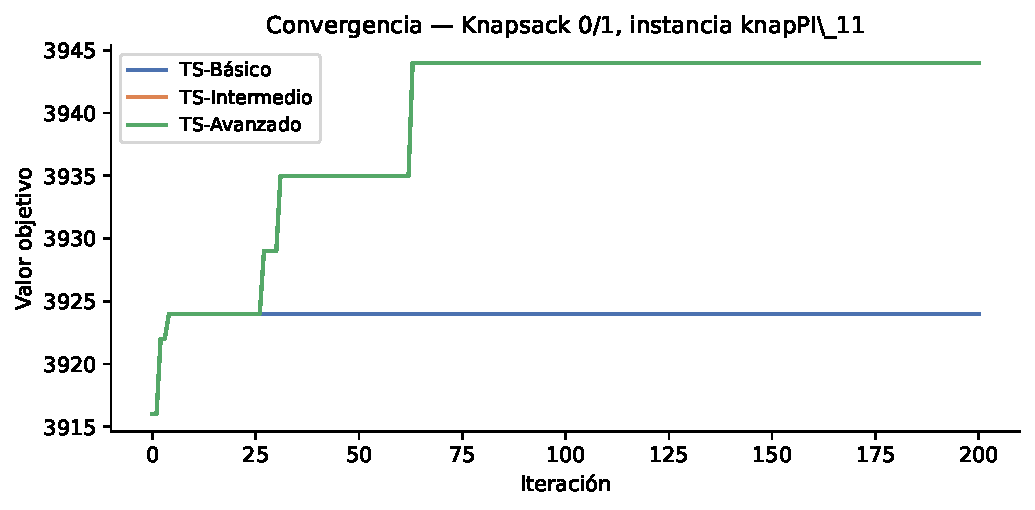
\includegraphics[width=\columnwidth]{figuras/convergencia_knapsack.pdf}
  \caption{Convergencia del GAP (\%) — Knapsack 0/1, instancia knapPI\_11
           (primeras 200 iteraciones).}
  \label{fig:conv_knapsack}
\end{figure}

Los tres niveles de TS logran GAPs inferiores al \SI{0.7}{\percent} en todas
las instancias, gracias a la pequeña dimensión del vecindario (flip de bit)
y a la buena solución inicial (greedy ratio).
TS-Avanzado no mejora significativamente sobre TS-Básico en este problema;
la memoria de frecuencia no contribuye positivamente cuando el espacio de
búsqueda es reducido y el vecindario es exhaustivo en cada iteración.
Como muestra la Figura~\ref{fig:conv_knapsack}, TS-Básico se estabiliza en
\SI{0.66}{\percent} tras cuatro iteraciones, mientras TS-Intermedio y
TS-Avanzado continúan mejorando hasta \SI{0.08}{\percent} en la iteración~73.

% ── TSP ─────────────────────────────────────────────────────────────────────
\subsection{TSP}

\begin{table}[t]
\caption{Resultados TSP: GAP\,(\%) y tiempo (s) — media(±$\sigma$) sobre 5 semillas}
\label{tab:tsp}
\centering
\footnotesize
\setlength{\tabcolsep}{3pt}
\begin{tabular}{lcccccc}
\toprule
 & \multicolumn{3}{c}{\textbf{GAP (\%) $\bar{x}$($\pm\sigma$)}}
 & \multicolumn{3}{c}{\textbf{Tiempo (s) $\bar{x}$}} \\
\cmidrule{2-4}\cmidrule{5-7}
\textbf{Instancia} & B & I & A & B & I & A \\
\midrule
berlin52 & 3.91(0.00) & 3.91(0.00) & 2.70(0.23)  &  0.86 &  1.75 &  3.54 \\
eil51 & 1.64(0.00) & 1.46(0.26) & 0.56(0.13)  &  0.70 &  1.56 &  3.56 \\
eil76 & 2.60(0.00) & 1.45(0.65) & 1.15(0.50)  &  1.76 &  3.51 &  7.72 \\
kroA100 & 2.99(0.00) & 2.99(0.00) & 0.76(0.03)  &  3.16 &  6.89 & 13.46 \\
kroB100 & 0.94(0.00) & 0.94(0.00) & 0.94(0.00)  &  3.08 &  6.76 & 13.67 \\
\midrule
\textbf{Media} & \textbf{2.42} & \textbf{2.15} & \textbf{1.22}
               & \textbf{1.91} & \textbf{4.09} & \textbf{8.39} \\
\bottomrule
\multicolumn{7}{l}{\scriptsize B=Básico, I=Intermedio, A=Avanzado. Formato: $\bar{x}$($\pm\sigma$)}
\end{tabular}
\end{table}

\begin{figure}[t]
  \centering
  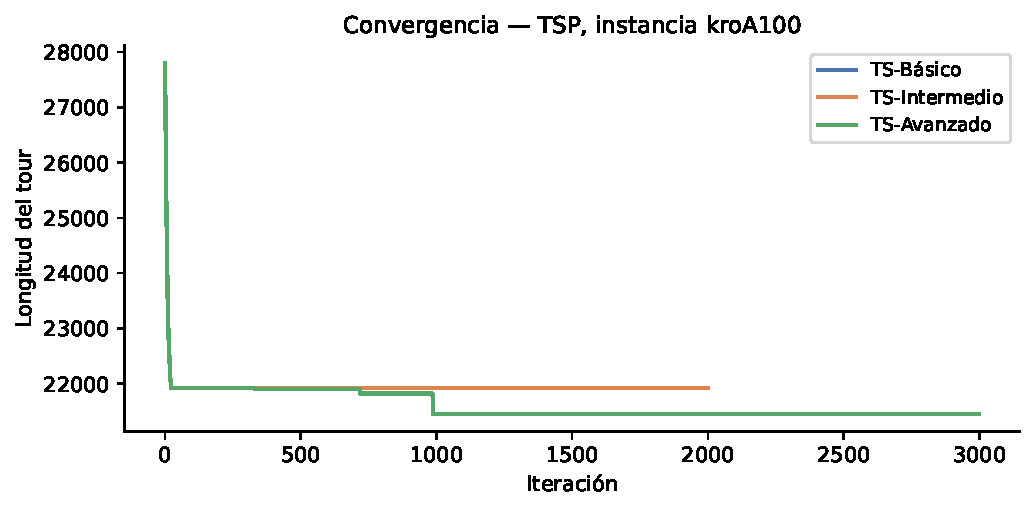
\includegraphics[width=\columnwidth]{figuras/convergencia_tsp.pdf}
  \caption{Convergencia del GAP (\%) — TSP, instancia kroA100.}
  \label{fig:conv_tsp}
\end{figure}

La TS-Básica obtiene GAPs de entre \SI{0.94}{\percent} y \SI{3.91}{\percent}.
TS-Intermedio mejora marginalmente gracias a la lista dinámica.
La mejora más notable se aprecia en TS-Avanzado, que incorpora perturbación
\emph{double-bridge}
(4-opt)~\cite{martin1992large,johnson1997traveling} al reinicio: para
\texttt{kroA100} el GAP cae de \SI{2.99}{\percent} a \SI{0.76}{\percent}.
El doble puente permite escapar de cuencas de atracción sin ser capturado
de nuevo por la lista tabú.
La Figura~\ref{fig:conv_tsp} ilustra la caída escalonada del GAP.

% ── CVRP ────────────────────────────────────────────────────────────────────
\subsection{CVRP}

\begin{table}[t]
\caption{Resultados CVRP: GAP\,(\%) y tiempo (s) — media(±$\sigma$) sobre 5 semillas}
\label{tab:cvrp}
\centering
\footnotesize
\setlength{\tabcolsep}{3pt}
\begin{tabular}{lcccccc}
\toprule
 & \multicolumn{3}{c}{\textbf{GAP (\%) $\bar{x}$($\pm\sigma$)}}
 & \multicolumn{3}{c}{\textbf{Tiempo (s) $\bar{x}$}} \\
\cmidrule{2-4}\cmidrule{5-7}
\textbf{Instancia} & B & I & A & B & I & A \\
\midrule
vrpnc1 & 26.26(0.00) & 7.94(0.00) & 6.69(1.14)  &  0.44 &  1.49 & 12.88 \\
vrpnc2 & 16.74(0.00) & 8.67(0.00) & 5.03(0.75)  &  1.03 &  2.56 & 27.40 \\
vrpnc3 & 14.95(0.00) & 5.59(0.00) & 4.64(0.75)  &  3.36 & 12.46 & 75.24 \\
vrpnc4 & 18.94(0.00) & 8.70(0.00) & 9.16(0.14)  &  6.88 & 20.32 & 161.47 \\
\midrule
\textbf{Media} & \textbf{19.22} & \textbf{7.72} & \textbf{6.38}
               & \textbf{2.93} & \textbf{9.21} & \textbf{69.25} \\
\bottomrule
\multicolumn{7}{l}{\scriptsize B=Básico, I=Intermedio, A=Avanzado. Formato: $\bar{x}$($\pm\sigma$)}
\end{tabular}
\end{table}

\begin{figure}[t]
  \centering
  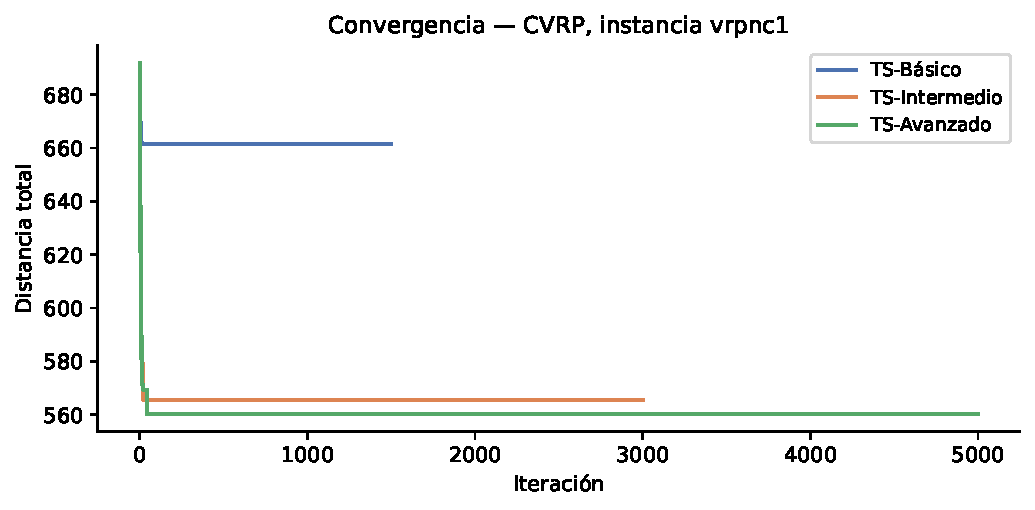
\includegraphics[width=\columnwidth]{figuras/convergencia_vrp.pdf}
  \caption{Convergencia del GAP (\%) — CVRP, instancia vrpnc1.}
  \label{fig:conv_vrp}
\end{figure}

Este es el problema donde la progresión de niveles tiene mayor impacto.
TS-Básico alcanza GAPs de hasta \SI{26.26}{\percent} en \texttt{vrpnc1},
reflejo de la dificultad de balancear rutas con un operador de reubicación
simple.
TS-Intermedio introduce intra-2opt inter-ruta, reduciendo el GAP promedio
a \SI{7.72}{\percent}.
TS-Avanzado añade frecuencia por cliente y penalización adaptativa, obteniendo
\SI{6.38}{\percent} promedio.
Para instancias grandes (\texttt{vrpnc3}, \texttt{vrpnc4}) el tiempo de
cómputo fue el principal limitante; con más iteraciones se esperaría mayor
mejora.
En particular, \texttt{vrpnc4} (150 clientes) presenta una inversión:
TS-Avanzado (\SI{9.16}{\percent}) no supera a TS-Intermedio (\SI{8.70}{\percent}),
posiblemente porque la penalización adaptativa sobrepondera clientes
muy visitados en instancias con alta densidad de rutas.
La Figura~\ref{fig:conv_vrp} evidencia las diferencias en velocidad y
profundidad de convergencia entre los tres niveles.

% ── Flowshop ────────────────────────────────────────────────────────────────
\subsection{Permutation Flowshop}

\begin{table}[t]
\caption{Resultados Flowshop: GAP\,(\%) y tiempo (s) — media(±$\sigma$) sobre 5 semillas}
\label{tab:flowshop}
\centering
\footnotesize
\setlength{\tabcolsep}{3pt}
\begin{tabular}{lcccccc}
\toprule
 & \multicolumn{3}{c}{\textbf{GAP (\%) $\bar{x}$($\pm\sigma$)}}
 & \multicolumn{3}{c}{\textbf{Tiempo (s) $\bar{x}$}} \\
\cmidrule{2-4}\cmidrule{5-7}
\textbf{Instancia} & B & I & A & B & I & A \\
\midrule
ta001 & 0.63(0.00) & 0.52(0.24) & 0.52(0.24)  &  0.84 &  1.72 &  1.88 \\
ta011 & 1.71(0.00) & 1.64(0.67) & 1.47(0.43)  &  1.30 &  2.85 &  3.75 \\
ta021 & 1.39(0.00) & 1.63(0.51) & 1.85(0.28)  &  2.74 &  5.68 &  6.30 \\
ta031 & 0.18(0.00) & 0.18(0.00) & 0.18(0.00)  &  4.78 &  9.68 & 11.91 \\
ta041 & 4.78(0.00) & 4.75(0.09) & 4.74(0.09)  &  9.01 & 17.55 & 21.80 \\
\midrule
\textbf{Media} & \textbf{1.74} & \textbf{1.74} & \textbf{1.75}
               & \textbf{3.73} & \textbf{7.50} & \textbf{9.13} \\
\bottomrule
\multicolumn{7}{l}{\scriptsize B=Básico, I=Intermedio, A=Avanzado. Formato: $\bar{x}$($\pm\sigma$)}
\end{tabular}
\end{table}

\begin{figure}[t]
  \centering
  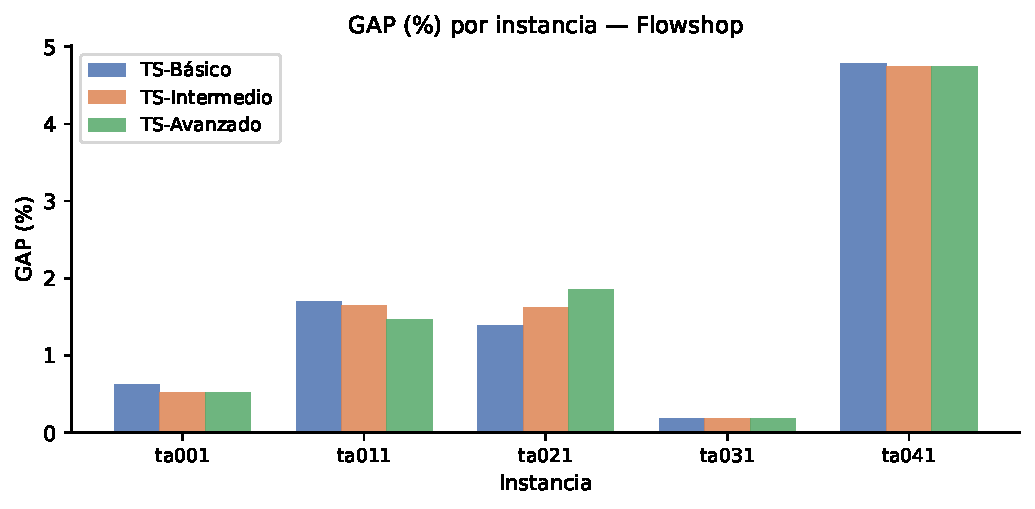
\includegraphics[width=\columnwidth]{figuras/convergencia_flowshop.pdf}
  \caption{GAP medio (\%) por instancia — Flowshop.}
  \label{fig:conv_flowshop}
\end{figure}

Los tres niveles obtienen GAPs medios muy similares:
\SI{1.74}{\percent}, \SI{1.74}{\percent} y \SI{1.75}{\percent}.
La heurística NEH entrega una solución inicial de buena calidad y la
vecindad de swap adyacente la mejora poco: los GAPs por instancia van de
\SI{0.18}{\percent} a \SI{4.78}{\percent}.
Para \texttt{ta041} (50 trabajos × 10 máquinas) el GAP se mantiene en
\SI{4.78}{\percent} para TS-Básico, \SI{4.75}{\percent} para TS-Intermedio y
\SI{4.74}{\percent} para TS-Avanzado; ello sugiere que la vecindad de swap
adyacente resulta limitada para explorar el espacio de búsqueda dentro del
presupuesto de iteraciones empleado; una vecindad de inserción podría
mejorar la solución a costa de tiempo computacional.
La Figura~\ref{fig:conv_flowshop} muestra el GAP medio por instancia: las
diferencias entre niveles son pequeñas y no siguen un orden fijo.
Los BKS de estas cinco instancias son makespan
óptimos~\cite{taillard1993benchmarks}; por ello, ningún GAP es negativo.
La Figura~\ref{fig:repr_soluciones} esquematiza cómo se representan las
soluciones que entrega cada algoritmo (archivo \texttt{solucion.txt} de
cada experimento).

\begin{figure}[t]
  \centering
  \begin{tikzpicture}[
      lab/.style={font=\scriptsize\bfseries, anchor=west},
      sol/.style={font=\scriptsize\ttfamily, anchor=west},
      celda/.style={draw, minimum width=0.42cm, minimum height=0.42cm,
                    font=\scriptsize\ttfamily, inner sep=1pt}]
    % Knapsack: vector binario
    \node[lab] at (0, 4.0) {Knapsack};
    \foreach \v/\i in {1/0, 0/1, 1/2, 1/3, 0/4, 1/5}
      \node[celda, fill={\ifnum\v=1 gray!25\else white\fi}]
        at (2.3 + \i*0.42, 4.0) {\v};
    \node[sol] at (5.2, 4.0) {$x_i \in \{0,1\}^n$};
    % TSP: tour
    \node[lab] at (0, 3.2) {TSP};
    \node[sol] at (2.1, 3.2)
      {0 $\to$ 3 $\to$ 1 $\to$ 4 $\to$ 2 $\to$ 0 \quad (tour)};
    % CVRP: rutas
    \node[lab] at (0, 2.4) {CVRP};
    \node[sol] at (2.1, 2.4)
      {$R_1$: 0-2-5-0;\ \ $R_2$: 0-1-4-3-0 \quad ($K$ rutas)};
    % Flowshop: permutación
    \node[lab] at (0, 1.6) {Flowshop};
    \node[sol] at (2.1, 1.6)
      {$\sigma = (3, 1, 4, 2, 5)$ \quad (permutación única)};
    % Job Shop: secuencia por máquina
    \node[lab] at (0, 0.8) {Job Shop};
    \node[sol] at (2.1, 0.8)
      {$M_1$: J1-J3-J2;\ \ $M_2$: J2-J1-J3;\ \ldots};
    \node[sol] at (2.1, 0.35)
      {(orden por máquina, cf.\ Fig.~\ref{fig:jobshop_gantt})};
  \end{tikzpicture}
  \caption{Representación de las soluciones en cada problema: vector
           binario (Knapsack), tour (TSP), conjunto de rutas (CVRP),
           permutación de trabajos (Flowshop) y orden de operaciones por
           máquina (Job Shop).}
  \label{fig:repr_soluciones}
\end{figure}

% ── Job Shop ────────────────────────────────────────────────────────────────
\subsection{Job Shop}

\begin{table}[t]
\caption{Resultados Job Shop: GAP\,(\%) y tiempo (s) — media(±$\sigma$) sobre 5 semillas}
\label{tab:jobshop}
\centering
\footnotesize
\setlength{\tabcolsep}{3pt}
\begin{tabular}{lcccccc}
\toprule
 & \multicolumn{3}{c}{\textbf{GAP (\%) $\bar{x}$($\pm\sigma$)}}
 & \multicolumn{3}{c}{\textbf{Tiempo (s) $\bar{x}$}} \\
\cmidrule{2-4}\cmidrule{5-7}
\textbf{Instancia} & B & I & A & B & I & A \\
\midrule
ft10 & 19.78(0.00) & 20.43(0.74) & 19.59(0.91)  &  8.49 &  3.11 &  4.53 \\
la01 & 1.80(0.00) & 2.25(1.24) & 1.65(0.57)  &  4.12 &  1.46 &  2.23 \\
la06 & 6.05(0.00) & 0.00(0.00) & 0.00(0.00)  & 13.28 &  4.73 &  6.91 \\
la11 & 0.00(0.00) & 1.33(1.57) & 0.00(0.00)  & 28.39 & 10.13 & 15.39 \\
la21 & 16.83(0.00) & 17.19(0.87) & 16.35(1.33)  & 25.98 & 10.12 & 14.34 \\
\midrule
\textbf{Media} & \textbf{8.89} & \textbf{8.24} & \textbf{7.52}
               & \textbf{16.05} & \textbf{5.91} & \textbf{8.68} \\
\bottomrule
\multicolumn{7}{l}{\scriptsize B=Básico, I=Intermedio, A=Avanzado. Formato: $\bar{x}$($\pm\sigma$)}
\end{tabular}
\end{table}

\begin{figure}[t]
  \centering
  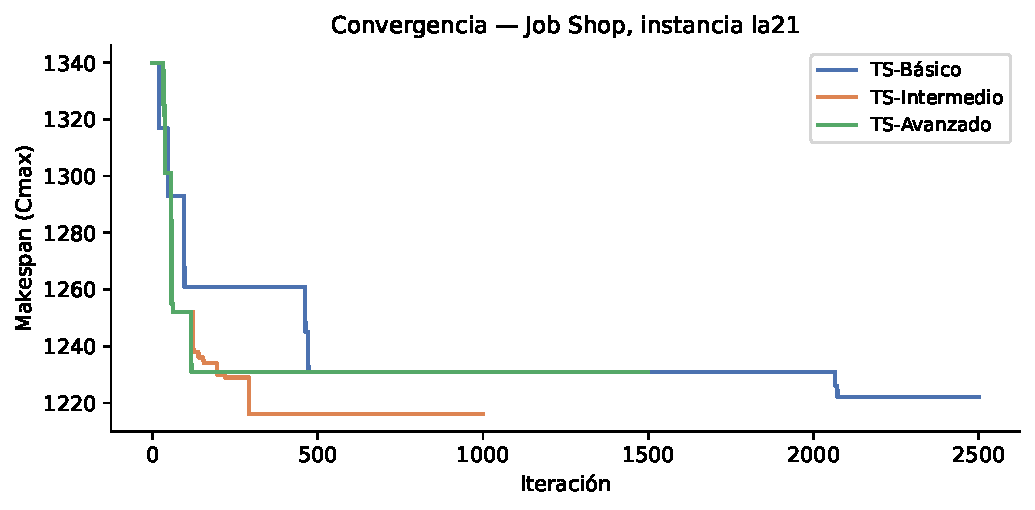
\includegraphics[width=\columnwidth]{figuras/convergencia_jobshop.pdf}
  \caption{Convergencia del GAP (\%) — Job Shop, instancia la21.}
  \label{fig:conv_jobshop}
\end{figure}

Job Shop es el problema más difícil del conjunto: \texttt{la21} y
\texttt{ft10} presentan GAPs de \SI{16.35}{\percent}–\SI{20.43}{\percent},
consistentes con la dificultad conocida de estos
benchmarks~\cite{nowicki1996fast}, y la
Figura~\ref{fig:conv_jobshop} confirma la estabilización temprana del GAP
en \texttt{la21}.
Las regresiones puntuales de TS-Intermedio (\texttt{la11}, \texttt{ft10})
y su alta varianza sugieren que la lista tabú dinámica y la penalización
de frecuencia son inestables en espacios de búsqueda muy accidentados.
En cambio, las instancias pequeñas (\texttt{la01}, \texttt{la06}) alcanzan
GAPs de \SI{0.00}{\percent}–\SI{2.25}{\percent}, al validar el decodificador
de Giffler-Thompson~\cite{giffler1960algorithms}.
TS-Intermedio es más rápido que TS-Básico ($5.91$\,s vs.\ $16.05$\,s)
porque emplea $T_{\max}=1\,000$ iteraciones frente a $2\,500$
(véase Tabla~\ref{tab:parametros}), decisión de diseño que mantiene tiempos
comparables dado el mayor costo por iteración de la lista dinámica.

% ── Análisis global ──────────────────────────────────────────────────────────
\subsection{Análisis global}

\begin{table}[tb]
\caption{GAP promedio (\%) y tiempo promedio (s) por problema y algoritmo}
\label{tab:consolidada}
\centering
\footnotesize
\setlength{\tabcolsep}{4pt}
\begin{tabular}{lcccccc}
\toprule
 & \multicolumn{2}{c}{\textbf{TS-Básico}}
 & \multicolumn{2}{c}{\textbf{TS-Intermedio}}
 & \multicolumn{2}{c}{\textbf{TS-Avanzado}} \\
\cmidrule{2-3}\cmidrule{4-5}\cmidrule{6-7}
\textbf{Problema} & GAP\% & T(s) & GAP\% & T(s) & GAP\% & T(s) \\
\midrule
Knapsack    & 0.22  & 0.01  & 0.13  & 0.02  & 0.10  & 0.07  \\
TSP         & 2.42  & 1.91  & 2.15  & 4.09  & 1.22  & 8.39  \\
CVRP        & 19.22  & 2.93  & 7.72  & 9.21  & 6.38  & 69.25  \\
Flowshop    & 1.74  & 3.73  & 1.74  & 7.50  & 1.75  & 9.13  \\
Job Shop    & 8.89  & 16.05  & 8.24  & 5.91  & 7.52  & 8.68  \\
\midrule
\textbf{Global} & \textbf{6.50} & -- & \textbf{4.00} & -- & \textbf{3.40} & -- \\
\bottomrule
\end{tabular}
\end{table}

El Cuadro~\ref{tab:consolidada} sintetiza los resultados a nivel de problema.
El costo computacional crece con el nivel, pero de forma moderada:
TS-Avanzado requiere en promedio $3.9\times$ el tiempo de TS-Básico,
mientras que la reducción de GAP es del \SI{48}{\percent} relativo.

% -----------------------------------------------------------------------
\section{Conclusiones y Trabajo Futuro}
\label{sec:conclusiones}

Se presentó un repositorio reproducible con 15 implementaciones de
Búsqueda Tabú (tres niveles) sobre cinco problemas clásicos de optimización
combinatoria, con experimentación automatizada.

\subsection*{Puntos de interés a nivel de implementación}

\begin{enumerate}
  \item \textbf{La progresión de niveles reduce el GAP global cerca de la
    mitad.}
    La transición de TS-Básico a TS-Avanzado reduce el GAP global de
    \SI{6.50}{\percent} a \SI{3.40}{\percent}, siendo CVRP el problema
    más beneficiado (reducción del \SI{67}{\percent} relativo).

  \item \textbf{El primer salto de complejidad concentra la mayor parte de
    la mejora.}
    TS-Intermedio reduce el GAP en 2.50\,pp respecto a
    TS-Básico, y TS-Avanzado reduce adicionalmente 0.60\,pp respecto a TS-Intermedio gracias a los mecanismos de largo plazo.

  \item \textbf{La perturbación informada es crítica en TSP.}
    El reinicio \emph{double-bridge} (4-opt) en TS-Avanzado es responsable
    de la mayor mejora individual observada: \SI{2.21}{\percent} de
    reducción en \texttt{kroA100}.

  \item \textbf{En Flowshop los tres niveles rinden de forma similar.}
    La heurística constructiva NEH entrega una solución inicial de buena
    calidad y los tres niveles de TS la mejoran poco (GAP medio entre
    \SI{1.74}{\percent} y \SI{1.75}{\percent}); el rendimiento en este
    problema está limitado por la vecindad de swap adyacente.

  \item \textbf{Job Shop es el problema más difícil del conjunto.}
    Los GAPs elevados en \texttt{la21} y \texttt{ft10} confirman la
    dificultad inherente del problema y la necesidad de vecindades más
    ricas (e.g., movimientos en el grafo de disyunción~\cite{balas1998one}).
\end{enumerate}

\subsection*{Trabajo futuro}

\begin{itemize}
  \item Incorporar modelos exactos (MILP) para las instancias de menor
    tamaño y comparar con los cotas inferiores.
  \item Implementar una cuarta configuración con TS poblacional
    (búsqueda tabú de trayectorias paralelas).
  \item Añadir instancias de mayor escala (e.g., TSP con 500+ ciudades,
    CVRP con 500+ clientes) y medir el escalado del GAP.
  \item Extender el repositorio a otros problemas como el de coloración
    de grafos o la mochila multidimensional.
  \item Automatizar la generación de figuras desde los cuadernos Jupyter
    e integrarlas directamente al PDF del artículo mediante \texttt{latexmk}.
\end{itemize}

En conclusión, la arquitectura progresiva de TS aquí validada permite
comprender el impacto incremental de cada mecanismo metaheurístico, y el
código publicado facilita su reproducción y extensión.


% -----------------------------------------------------------------------
% Balanceo de columnas en última página
\bibliographystyle{IEEEtran}
\bibliography{referencias}

\end{document}

